
\chapter{Bibliothèque de monitoring de la mémoire d'E-ACSL2C}
\label{sec:eacsl}

\chapterintro


Dans ce chapitre nous présentons notre implémentation du modèle mémoire des
programmes C qui permet d'exécuter les annotations \eacsl présentées dans
le chapitre~\ref{sec:runtime}.
Notre bibliothèque permet au greffon \eacsltoc de vérifier à l'exécution les
annotations \eacsl portant sur le modèle mémoire.

\eacsltoc traduit automatiquement un programme C annoté en un autre
programme C dont l'exécution échouera si une annotation n'est pas valide.
Si aucune annotation n'est violée, le comportement
du nouveau programme est exactement le même que celui du programme d'origine.
Ce greffon utilise notre bibliothèque afin de vérifier à l'exécution les
annotations \eacsl portant sur la mémoire.
Le greffon \eacsltoc lui-même n'étant pas le fruit de nos travaux
\cite{Delahaye/SAC13}, il ne sera pas présenté dans ce chapitre.

Nous présentons la bibliothèque en partie~\ref{sec:eacsl-impl}.
Au cours de nos travaux, nous avons mesuré la capacité de détection d'erreur de
notre implémentation et nous avons comparé les performances à l'exécution de
plusieurs choix d'implémentation.
Nous présentons les résultats de nos expérimentations en
partie~\ref{sec:eacsl-exp}.


\section{Architecture de la bibliothèque de monitoring de la mémoire}
\label{sec:eacsl-impl}


Les annotations présentées au chapitre~\ref{sec:runtime} prennent en paramètre
des adresses mémoire, et non des left-values.
La vérification de ces annotations nécessite donc une représentation du
{\em store} tel qu'il a été présenté dans la partie~\ref{sec:mem-model}, mais ne
nécessite pas de représenter l'environnement.

La figure~\ref{fig:mmodel-architecture} présente l'architecture générale de la
bibliothèque au moyen du graphe de dépendance des fonctions C les plus
importantes.
Une flèche $A \rightarrow B$ signifie que la fonction $A$ appelle la fonction
$B$.

\begin{figure}[h!]
  \centering
  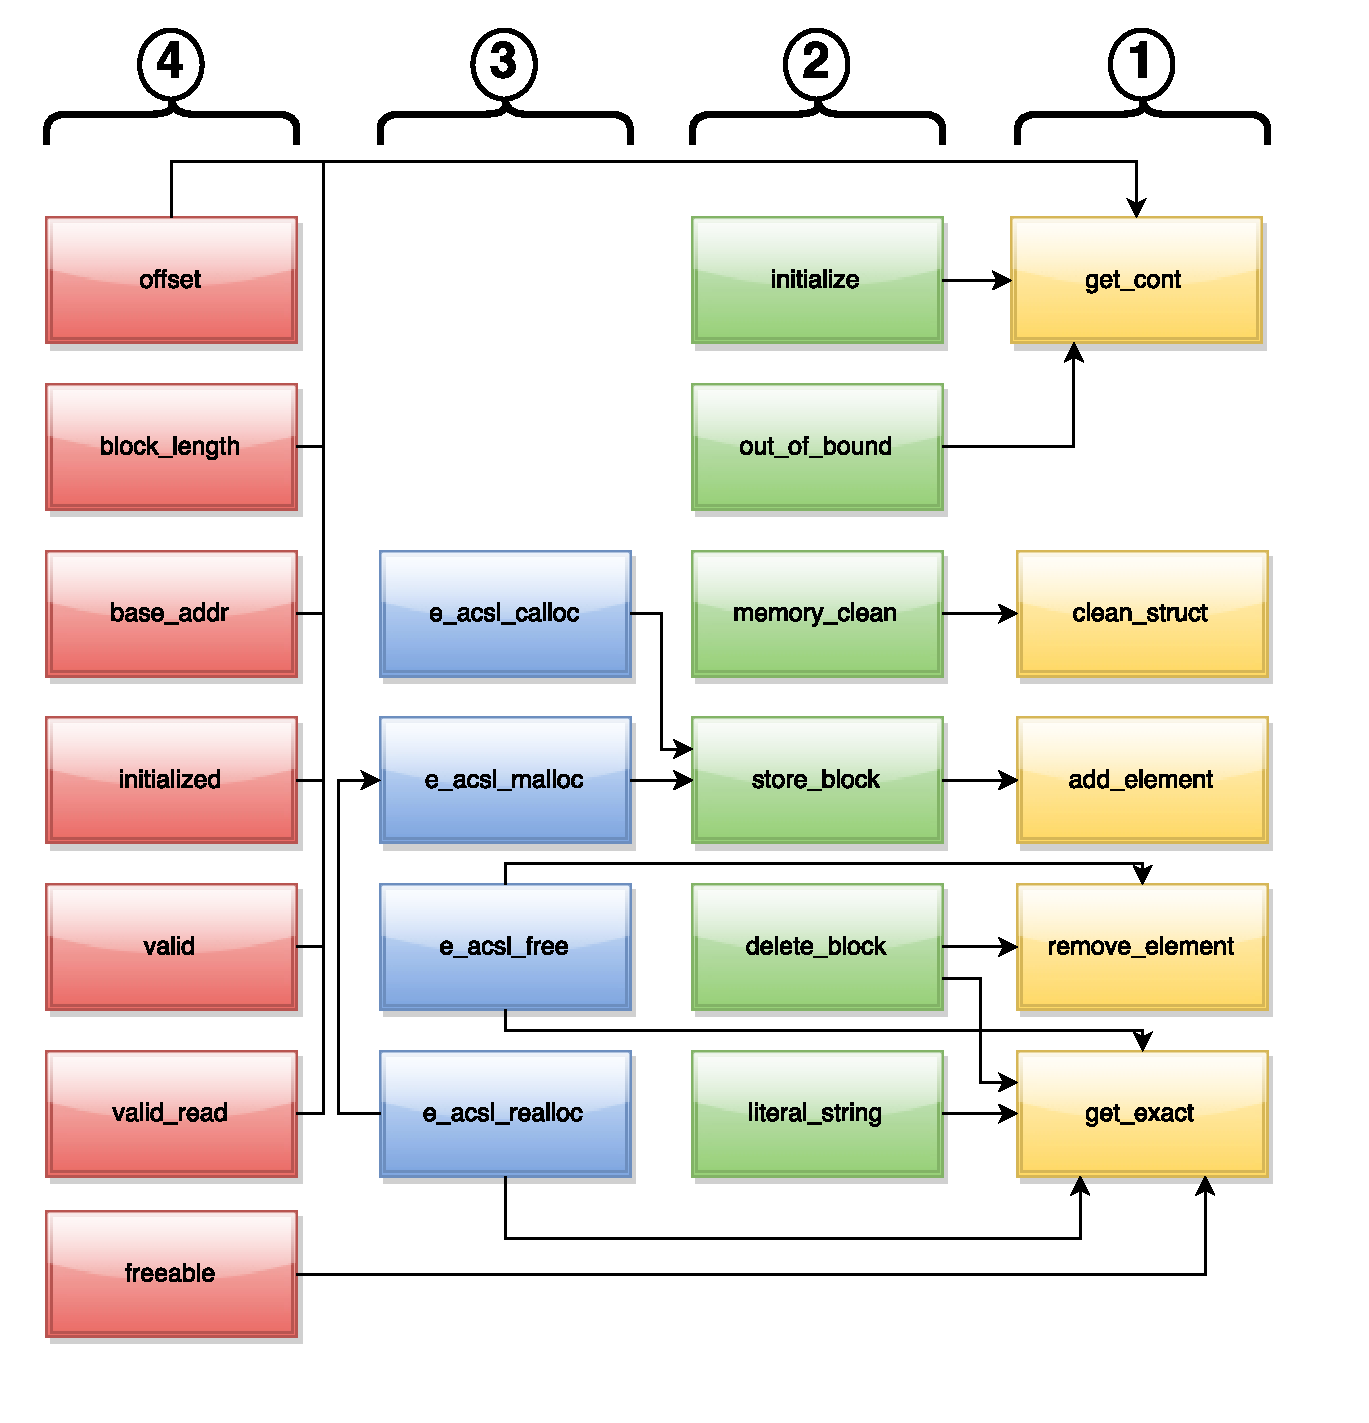
\includegraphics[scale=.55]{figures/mmodel_architecture.pdf}
  \vspace{-.8cm}
  \caption{Architecture de la bibliothèque de monitoring de la mémoire
    \label{fig:mmodel-architecture}}
\end{figure}

L'architecture comporte quatre niveaux, numérotés de \circled{1} à \circled{4}.
Les fonctions du niveau \circled{1} correspondent à l'implémentation de la
structure de données {\em store} (présentée au chapitre~\ref{sec:runtime})
gardant les informations à propos des blocs alloués.
Plusieurs implémentations sont fournies pour ces fonctions, correspondant à
différentes structures de données génériques : listes chaînées, arbres binaires
de recherche, Splay trees et Patricia tries.
La fonction \lstinline'get_exact' de la figure~\ref{fig:mmodel-architecture}
implémente l'algorithme~\ref{algo:get-exact}.
La fonction \lstinline'get_cont' implémente l'algorithme~\ref{algo:get-cont}.
La fonction \lstinline'add_element' implémente
l'algorithme~\ref{algo:add-block}.
La fonction \lstinline'remove_element' implémente
l'algorithme~\ref{algo:rem-block}.
Les fonctions du niveau \circled{2} servent à modifier le contenu du {\em store}
(ajout ou suppression d'élément, initialisation des éléments, etc.).
Les fonctions du niveau \circled{3} doivent être appelées en lieu et place des
fonctions de la bibliothèque standard associées (\lstinline'malloc', etc.).
Les fonctions \lstinline'e_acsl_malloc', \lstinline'e_acsl_calloc',
\lstinline'e_acsl_realloc' et \lstinline'e_acsl_free' de la
figure~\ref{fig:mmodel-architecture} correspondent respectivement aux fonctions
\lstinline'__malloc', \lstinline'__calloc',
\lstinline'__realloc' et \lstinline'__free' présentées au
chapitre~\ref{sec:runtime}.
Les fonctions du niveau \circled{4} permettent de calculer la valeur des
annotations \eacsl, elles retournent la valeur du terme ou du prédicat \eacsl
correspondant.
Ces fonctions ne modifient pas le contenu du {\em store}.
Les fonctions \lstinline'offset', \lstinline'block_length',
\lstinline'base_addr', \lstinline'initialized', \lstinline'valid' et
\lstinline'valid_read' de la figure~\ref{fig:mmodel-architecture} correspondent
respectivement aux fonctions \lstinline'__offset', \lstinline'__block_length',
\lstinline'__base_addr', \lstinline'__initialized', \lstinline'__valid' et
\lstinline'__valid_read' présentées au chapitre~\ref{sec:runtime}.

Les fonctions des niveaux \circled{2}, \circled{3} et \circled{4} sont
implémentées de manière indépendante à l'implémentation du {\em store} (niveau
\circled{1}).
Cette architecture facilite la conception des algorithmes, ainsi que la
comparaison d'efficacité des différentes implémentations du {\em store},
effectuée en partie~\ref{sec:eacsl-exp}.


\section{Expérimentations}
\label{sec:eacsl-exp}


Nous présentons maintenant les résultats de nos expérimentations visant à
évaluer la capacité de détection d'erreurs de la bibliothèque et la performance
à l'exécution des différents choix d'implémentation.


\subsection{Capacité de détection d'erreurs}


\begin{figure}
  \centering
  \begin{tabular}{c|c|c|c|c|c}
    & alarmes & mutants & équivalents & tués & \% erronés tués \\
    \hline
    fibonacci & 19  & 27 & 2 & 25 & 100\% \\
    \hline
    bubbleSort & 15  & 44 & 2 & 42 & 100\% \\
    \hline
    insertionSort & 10  & 39 & 3 & 36 & 100\% \\
    \hline
    binarySearch & 7 & 38 & 1 & 37 & 100\% \\
    \hline
    merge & 5 & 92 & 5 & 87 & 100\% \\
  \end{tabular}
  \caption{Capacité de détection d'erreurs
    \label{tab:mutation-exp}}
\end{figure}


Nous avons utilisé la technique de mutation pour évaluer la capacité de
détection d'erreurs en utilisant la vérification d'assertion à l'exécution avec
\framac.
Nous avons considéré 5 programmes écrits et annotés par nos soins.
Nous avons généré leurs {\em mutants} (en appliquant une {\em mutation} sur leur
code source) et leur avons appliqué la vérification à l'exécution.
Les mutations du programme incluent : modifications d'opérateurs arithmétiques
numériques, modifications d'opérateurs arithmétiques sur les pointeurs,
modifications d'opérateurs de comparaison et modifications d'opérateurs logiques
($et$ et $ou$).
L'outil de génération de test \pathcrawler \cite{\citepathcrawler} a été
utilisé pour produire les cas de test.
Chaque mutant a été instrumenté par \eacsltoc et exécuté sur chaque cas de test
pour vérifier que la spécification était satisfaite à l'exécution.
Les programmes d'origine passent toutes les vérifications à l'exécution.
Lorsqu'une violation d'une annotation a été reportée pour au moins un cas de
test, le mutant est considéré comme étant {\em tué}.
La figure~\ref{tab:mutation-exp} présente les résultats.
La première colonne contient les exemples étudiés.
La deuxième colonne contient le nombre d'annotations dans chaque programme.
Les colonnes suivantes contiennent le nombre de mutants générés, le nombre de
mutants équivalents à leur programme d'origine (décidé par analyse manuelle), le
nombre de mutants non-équivalents tués, et le pourcentage des mutants
non-équivalents tués lors de l'exécution.
Lors de ces expérimentations, tous les mutants non-équivalents erronés ont été
tués, ce qui témoigne de la précision et de la complétude de notre méthode.


\subsection{Performance des choix d'implémentation}


Pour évaluer la performance à l'exécution de notre implémentation de la
bibliothèque, nous avons effectué plus de 300 exécutions sur plus de 30
programmes, obtenus à partir d'une dizaine de programmes écrits et annotés par
nos soins.
Nous avons volontairement gardé des exemples plutôt courts (moins de 200 lignes
de code) car ils ont dû être annotés en \eacsl manuellement.

Nous avons mesuré le temps d'exécution du programme d'origine et du code
instrumenté par \eacsltoc avec différentes options, afin d'évaluer les
performances des différentes implémentations du {\em store} et des différentes
optimisations.


\textbf{Calcul du plus grand préfixe commun :} \\
Nous avons comparé deux implémentations de ce calcul, qui est utilisé par
l'implémentation du {\em store} utilisant des Patricia tries.
La première implémentation utilise un parcours linéaire de l'adresse (bit-à-bit,
de gauche à droite).
La seconde implémentation est une recherche dichotomique du meilleur préfixe
dans un tableau dont le contenu et les indices sont pré-calculés.
Elle implémente l'algorithme~\ref{algo:prefix} présenté en
partie~\ref{sec:mpgpc}.
Cette seconde implémentation s'est révélée en moyenne 2.7 fois plus rapide que
la première sur nos exemples.


\begin{figure}[h!]
  \begin{tikzpicture}
    \begin{axis}[axis y line=left,width=\textwidth,height=\textwidth,ymode=log,
        legend columns=2,xlabel={$N$},ylabel={temps (s.)},scaled ticks=false,
        x tick label style={rotate=90,anchor=east}, xlabel near ticks,
        xtick={1000,5000,10000,50000,100000}]
      \pgfplotstableread{data/table_eacsl_experiments_merge_sort.dat}
      \loadedtable;
      \addplot [color=red,ultra thick] table[x=N,y=list] {\loadedtable}
      node[above,pos=1] {list};

      \addplot [color=red,dashed,ultra thick]
      table[x=N,y=list-DFA] {\loadedtable}
      node[below,left,pos=1,yshift=-.5cm] {list-AS};

      \addplot [color=blue,ultra thick] table[x=N,y=bst] {\loadedtable}
      node[above,right,pos=1] {bst};

      \addplot [color=blue,dashed,ultra thick]
      table[x=N,y=bst-DFA] {\loadedtable}
      node[above,right,pos=1] {bst-AS};

      \addplot [color=greenv,ultra thick] table[x=N,y=Pt] {\loadedtable}
      node[above,left,pos=1,xshift=-1.4cm] {Pt};

      \addplot [color=greenv,dashed,ultra thick]
      table[x=N,y=Pt-DFA] {\loadedtable}
      node[above,left,pos=1] {Pt-dicho};

      \addplot [color=orange,ultra thick] table[x=N,y=Pt-opti] {\loadedtable}
      node[below,right,pos=1,yshift=-.5cm,xshift=-1.2cm] {Pt-AS};

      \addplot [color=orange,dashed,ultra thick]
      table[x=N,y=Pt-opti-DFA] {\loadedtable}
      node[above,left,pos=1] {Pt-dicho-AS};

      \addplot [color=violet,ultra thick] table[x=N,y=St] {\loadedtable}
      node[below,right,pos=1] {St};

      \addplot [color=violet,dashed,ultra thick]
      table[x=N,y=St-DFA] {\loadedtable}
      node[below,right,pos=1,yshift=-.7cm] {St-AS};

      \legend{list,list-AS,bst,bst-AS,Pt,Pt-dicho,Pt-AS,Pt-dicho-AS,St,St-AS}
    \end{axis}
  \end{tikzpicture}
  \vspace{-.8cm}
  \caption{Comparaison du temps d'exécution des différentes implémentations du
    {\em store} sur un tri fusion de $N$ éléments
    \label{fig:mmodel-exp}}
\end{figure}


\textbf{Implémentation du {\em store} :}\\
Pour déterminer quelle implémentation du {\em store} est la plus appropriée,
nous avons comparé quatre implémentations utilisant des chaînées (notées $list$
sur les figures~\ref{fig:mmodel-exp} et~\ref{tab:mmodel-exp}), des arbres
binaires de recherche non équilibrés (notés $bst$), des arbres binaires de
recherche équilibrés (Splay trees~\cite{Sleator/85}, notés $St$) et des Patricia
tries.
Nous distinguons deux implémentations à base de Patricia tries : la première
(notée $Pt$) où l'algorithme de recherche du masque du plus grand préfixe commun
est implémenté de manière linéaire, et la seconde (notée $Pt-dicho$) où la
recherche du masque du plus grand préfixe commun est implémentée en utilisant
l'algorithme~\ref{algo:prefix} présenté en partie~\ref{sec:mpgpc}.

Le greffon \eacsltoc utilise une analyse statique qui permet de n'instrumenter
que ce qui est nécessaire.
Une analyse dataflow arrière est faite afin de déterminer une sur-approximation
des left-values dont l'instrumentation est nécessaire pour chaque annotation,
ce qui réduit le  nombre de left-values surveillées à l'exécution.
Cette analyse n'étant pas le fruit de nos travaux (section 6 de
\cite{\citeeacsltoc}), nous ne la présentons pas ici.
Nous en profitons néanmoins pour mesurer l'impact qu'a cette analyse pour
chaque implémentation du {\em store} dans nos expérimentations.
Ces mesures sont respectivement dénotées pour chaque implémentation
$list$-$AS$, $bst$-$AS$, $St$-$AS$, $Pt$-$AS$ et $Pt$-$dicho$-$AS$.

La figure~\ref{fig:mmodel-exp} représente graphiquement le temps (en secondes)
passé par chaque implémentation du {\em store} sur un tri fusion pour $N$ =
1000, 5000, 10000, 50000 et 100000 éléments.
Les données chiffrées sont dans les cinq dernières lignes de la
figure~\ref{tab:mmodel-exp}.
Nous voyons sur la figure~\ref{fig:mmodel-exp} que, sur cet exemple, les
implémentations du {\em store} sont, de la plus efficace à la moins efficace :
Splay tree, Patricia trie ``dicho'', Patricia trie ``linéaire'', arbre binaire
de recherche et liste chaînée.
Pour chacune de ces implémentations, l'utilisation de l'analyse statique
dataflow apporte un gain d'efficacité.
Les meilleures performances de l'implémentation à base de Splay tree sont dues à
la nature de l'exemple (un tri fusion) où il y a de nombreux accès mémoire
consécutifs sur même bloc, ce qui joue en faveur des Splay tree : le dernier
élément accédé est remonté à la racine de l'arbre.
La figure~\ref{tab:mmodel-exp} prend en compte un plus large spectre de
programmes, ce qui permet de nuancer ces résultats.

La figure~\ref{tab:mmodel-exp} présente les résultats des expérimentations
comparant les différentes implémentations du {\em store} et du calcul du plus
grand préfixe commun sur de nombreux exemples.
La première colonne du tableau contient les exemples étudiés.
$bS_{10000}$ est une recherche binaire dans un tableau de 10000 éléments.
$iS_{10000}$ est un tri par insertion d'un tableau de 10000 éléments.
$mM_{n^2}$ est une multiplication de matrices $n \times n$. mI$_{n^2}$ contient
des calculs matriciels (dont inversion et multiplication) sur des  matrices
$n \times n$.
$qS_n$ est un tri rapide sur un tableau de $n$ éléments.
$bbS_{10000}$ est un tri à bulle sur un tableau à 10000 éléments.
$m_{30000}$ est une fusion de deux listes chaînées de 10000 et 20000 éléments.
$Rbt_{10000}$ est une insertion/suppression de 10000 éléments dans un arbre rouge
et noir.
$mS_n$ est un tri fusion d'une liste chaînée de $n$ éléments.
La ligne supplémentaire ``+ RTE'' de chaque exemple correspond à l'exemple après
application du greffon \rte qui génère des assertions qui sont vraies si le
programme ne contient pas d'erreur à l'exécution.
Nous appelons ces assertions à vérifier des ``alarmes''.

La colonne $\danger$ contient le nombre d'annotations du programme (celles
ajoutées manuellement et celles générées par le greffon \rte).
La colonne $\emptyset$ contient le temps d'exécution du programme original.
Tous les temps d'exécution sont mesurés en secondes.
Un temps d'exécution est noté $\infty$ quand il dépasse 24 heures.
Les colonnes $list$ à $St$-$AS$ contiennent le temps d'exécution du programme
pour chaque implémentation du {\em store}.
Le temps d'analyse du programme sans instrumentation avec le débogueur
\valgrind~\cite{\citevalgrind} est indiqué dans la dernière colonne.

Nous remarquons que le temps d'exécution de \valgrind n'est pas comparable avec
celui de notre bibliothèque, cela s'explique simplement par le fait que celui-ci
ne prend pas en compte la spécification \eacsl, et se contente de vérifier des
propriétés comme l'absence d'erreur de segmentation ou l'absence de fuite de
mémoire.
En effet, notre démarche vise à supporter au maximum les annotations \eacsl,
ce qui nécessite un monitoring plus lourd.

Les résultats de nos expérimentations confirment nos hypothèses, à savoir :

\begin{itemize}
\item[\textbf{H1}]
  le Patricia trie est la structure de données la plus appropriée pour
  l'implémentation du {\em store};

\item[\textbf{H2}]
  notre optimisation de la recherche du masque du plus grand préfixe commun par
  recherche dichotomique et l'utilisation d'indices pré-calculés entraîne un
  vrai gain de performance;

\item[\textbf{H3}]
  l'utilisation d'une analyse statique visant à réduire l'instrumentation
  du programme permet de réduire le temps d'exécution de manière efficace.
\end{itemize}

Concernant \textbf{H1}, la figure~\ref{tab:mmodel-exp} montre que
l'implémentation du {\em store} par un Patricia trie est la plus efficace.
La version utilisant les Splay trees offre des performances comparables (ou
légèrement meilleures, jusqu'à 3 fois) sur les exemples contenant de fréquents
accès mémoire consécutifs au même bloc dans le {\em store}, comme c'est le cas
du tri fusion (voir la figure~\ref{fig:mmodel-exp}).
En revanche, sur des exemples où les accès mémoire consécutifs ne se font pas
sur le même bloc (une multiplication de matrices dans notre exemple), les
performances sont beaucoup moins bonnes (jusqu'à 500 fois).
Ceci est dû à la nature des Splay trees : le dernier élément accédé est remonté
à la racine de l'arbre.
En moyenne, l'implémentation à base de Patricia trie est 2500 fois plus rapide
que l'implémentation à base de listes chaînées, 200 fois plus rapide que celle
utilisant les arbres binaires de recherche, et 27 fois plus rapide que celle se
basant sur les Splay trees.

Concernant \textbf{H2}, la figure~\ref{tab:mmodel-exp} montre que la version
dichotomique de la recherche du masque du plus grand préfixe commun est toujours
plus efficace qu'une recherche linéaire.
Elle est en moyenne 3 fois plus rapide que cette dernière.

Concernant \textbf{H3}, nos résultats montrent que l'utilisation d'une analyse
statique visant à réduire l'instrumentation du programme entraîne un gain de
performance.
En effet, pour chacune des implémentations du {\em store}, l'analyse statique
permet de réduire le temps d'exécution.
L'exécution après analyse statique peut être jusqu'à 200 fois plus rapide sur
certains exemples.
Elle permet notamment de ne pas observer de {\em timeout} pour les listes
chaînées et les arbres binaires de recherche sur l'exemple du tri fusion de
50000 éléments.


\section*{Conclusion du chapitre}


Dans ce chapitre nous avons présenté l'architecture de l'implémentation de la
bibliothèque de monitoring de la mémoire, dont les algorithmes et les principes
théoriques ont été traités dans le chapitre~\ref{sec:runtime}.

Nous avons présenté les résultats de nos expérimentations visant à
mesurer la capacité de détection d'erreurs et les performances à l'exécution de
nos implémentations.
Nous avons notamment comparé les performances de quatre implémentations du
{\em store}.
Nous avons également comparé deux implémentations de la recherche du masque du
plus grand préfixe commun, dans le cas où le {\em store} est implémenté en
utilisant un Patricia trie.
Enfin, nous avons mesuré l'impact de l'utilisation d'une analyse statique visant
à réduire l'instrumentation du programme (section 6 de \cite{\citeeacsltoc}),
pour chacune des implémentations du {\em store}.
Nos expérimentations ont mis en avant l'efficacité d'une implémentation du
{\em store} à base de Patricia trie.
Elles ont également montré qu'une recherche du masque du plus grand préfixe
commun par dichotomie (l'algorithme est présenté en partie~\ref{sec:mpgpc}) est
plus efficace qu'une recherche linéaire et que l'analyse statique permet
effectivement de réduire le temps de la vérification à l'exécution.

Le travail réalisé a permis de concevoir une méthode et un outil de vérification
à l'exécution des annotations \eacsl portant sur le modèle mémoire.
Nos travaux ont permis de déterminer expérimentalement quelles implémentations
du {\em store} et des différents algorithmes sont les plus efficaces pour notre
outil de vérification.
L'implémentation du {\em store} à base de Patricia trie et les différents
algorithmes présentés dans ce chapitre et dans le chapitre~\ref{sec:runtime}
sont intégrés à l'outil \eacsltoc~\cite{\citeeacsltoc}.


\begin{landscape}
  \begin{figure}[h]
    \centering
    \begin{footnotesize}
      \begin{tabular}{l|c|c|c|c|c|c|c|HHc|c|HHc|c|c|c}
  & $\danger$ & $\emptyset$ & list & list-AS & bst & bst-AS & Pt & mask$^1$ & sb$^1$ & Pt-dicho & Pt-AS & mask$^2$ & sb$^2$ & Pt-dicho-AS & St & St-AS & valgrind \\
  \hline
  bS$_{10000}$ &22 &\multirow{2}{*}{.01} &1.10 &0.50 &1.14 &0.64 &1.55 &99 &16 &1.55 &0.57 &0 &1 &0.55 &1.39 &0.61 &\multirow{2}{*}{0.27}\\
  + RTE &41 &&1.10 &0.51 &1.14 &0.62 &1.59 &109 &16 &1.59 &0.53 &0 &1 &0.53 &1.39 &0.64 &\\
  \hline
  iS$_{10000}$ &5 &\multirow{2}{*}{.12} &2.29 &0.12 &1.83 &0.12 &2.89 &170k &20k &2.91 &0.12 &0 &0 &0.12 &2.46 &0.12 &\multirow{2}{*}{2.81}\\
  + RTE &24 &&3.52 &1.27 &2.89 &1.26 &3.99 &170k &20k &3.86 &1.25 &0 &0 &1.25 &3.46 &1.30 &\\
  \hline
  mM$_{100^2}$ &0 &\multirow{2}{*}{.01} &2.29 &0.73 &2.94 &1.15 &0.14 &17k &1k &0.14 &0.10 &5k &612 &0.09 &1.07 &0.98 &\multirow{2}{*}{0.34}\\
  + RTE &82 &&13.17 &10.66 &21.92 &17.39 &2.78 &18k &1k &3.00 &2.64 &5k &612 &2.82 &75.97 &73.62 &\\
  \hline
  mM$_{150^2}$ &0 &\multirow{2}{*}{.01} &13.23 &3.96 &15.65 &6.20 &0.54 &21k &2k &0.51 &0.36 &9k &912 &0.35 &5.86 &5.64 &\multirow{2}{*}{0.48}\\
  + RTE &82 &&72.36 &58.48 &110.70 &90.43 &10.77 &24k &2k &9.01 &8.57 &9k &912 &8.75 &403.50 &398.60 &\\
  \hline
  mI$_{100^2}$ &2 &\multirow{2}{*}{.01} &22.51 &0.10 &7.74 &0.13 &0.09 &68k &5k &0.08 &0.01 &7k &609 &0.01 &0.19 &0.10 &\multirow{2}{*}{0.35}\\
  + RTE &155 &&28.96 &4.22 &13.67 &5.48 &0.54 &73k &5k &0.55 &0.53 &7k &611 &0.47 &26.37 &26.16 &\\
  \hline
  mI$_{150^2}$ &2 &\multirow{2}{*}{.02} &130.04 &0.34 &40.35 &0.45 &0.28 &99k &8k &0.27 &0.02 &12k &909 &0.02 &0.68 &0.34 &\multirow{2}{*}{0.47}\\
  + RTE &155 &&153.30 &21.54 &73.55 &29.94 &2.00 &105k &8k &1.90 &1.42 &12k &911 &1.53 &146.15 &145.80 &\\
  \hline
  qS$_{1000}$ &15 &\multirow{2}{*}{.01} &12.70 &2.08 &1.76 &0.59 &0.33 &1M &92k &0.06 &0.13 &683k &39k &0.02 &0.02 &0.01 &\multirow{2}{*}{0.27}\\
  + RTE &32 &&12.38 &2.13 &1.64 &0.56 &0.38 &1M &92k &0.12 &0.14 &727k &39k &0.04 &0.03 &0.02 &\\
  \hline
  qS$_{2000}$ &15 &\multirow{2}{*}{.01} &85.99 &11.31 &8.39 &2.78 &0.71 &3M &198k &0.14 &0.28 &1M &84k &0.05 &0.03 &0.02 &\multirow{2}{*}{0.27}\\
  + RTE &32 &&81.65 &11.15 &7.72 &2.67 &1.13 &4M &198k &0.48 &0.36 &1M &84k &0.13 &0.05 &0.02 &\\
  \hline
  bbS$_{10000}$ &4 &\multirow{2}{*}{.22} &13.78 &1.02 &16.84 &1.67 &117.47 &499M &49M &22.36 &1.57 &30 &7 &1.54 &8.80 &1.67 &\multirow{2}{*}{3.36}\\
  + RTE &16 &&23.08 &4.64 &30.69 &7.16 &107.05 &599M &49M &32.58 &7.26 &29 &7 &6.90 &17.29 &7.21 &\\
  \hline
  m$_{30000}$ &2 &\multirow{2}{*}{.01} &412.10 &11.38 &176.35 &11.01 &1.11 &5M &420k &0.26 &0.30 &1M &60k &0.06 &0.08 &0.01 &\multirow{2}{*}{0.45}\\
  + RTE &49 &&451.58 &101.33 &219.12 &94.80 &1.15 &5M &420k &0.29 &0.47 &2M &130k &0.14 &0.10 &0.05 &\\
  \hline
  Rbt$_{10000}$ &0 &\multirow{2}{*}{.01} &47.39 &0.28 &48.44 &0.27 &0.32 &1M &159k &0.09 &0.03 &151k &10k &0.01 &0.59 &0.01 &\multirow{2}{*}{0.51}\\
  + RTE &270 &&120.02 &101.69 &165.77 &145.20 &0.47 &1M &159k &0.30 &0.39 &979k &119k &0.27 &18.82 &19.59 &\\
  \hline
  mS$_{1000}$ &7 &\multirow{2}{*}{.01} &6.45 &0.34 &6.32 &0.11 &0.32 &1M &95k &0.07 &0.06 &331k &18k &0.01 &0.02 &0.01 &\multirow{2}{*}{0.27}\\
  + RTE &45 &&6.82 &1.35 &7.98 &0.38 &0.34 &1M &95k &0.10 &0.13 &701k &38k &0.04 &0.02 &0.01 &\\
  \hline
  mS$_{5000}$ &7 &\multirow{2}{*}{.01} &362.87 &11.00 &218.01 &3.43 &2.28 &11M &562k &0.76 &0.43 &2M &106k &0.09 &0.14 &0.03 &\multirow{2}{*}{0.27}\\
  + RTE &45 &&371.40 &50.94 &290.88 &10.34 &2.46 &11M &562k &0.80 &0.83 &4M &218k &0.22 &0.16 &0.08 &\\
  \hline
  mS$_{10000}$ &7 &\multirow{2}{*}{.01} &3624.01 &47.94 &1673.00 &16.10 &6.46 &23M &1M &2.75 &1.00 &5M &223k &0.21 &0.31 &0.08 &\multirow{2}{*}{0.27}\\
  + RTE &45 &&3406.43 &257.18 &2086.32 &46.22 &6.30 &23M &1M &2.66 &1.83 &9M &457k &0.51 &0.35 &0.18 &\\
  \hline
  mS$_{50000}$ &7 &\multirow{2}{*}{.01} &$\infty$ &3847.72 &$\infty$ &1100.93 &135.54 &146M &6M &111.22 &6.90 &33M &1M &1.65 &2.08 &0.58 &\multirow{2}{*}{0.63}\\
  + RTE &45 &&$\infty$ &25554.08 &$\infty$ &2781.90 &118.86 &145M &6M &95.74 &11.64 &54M &2M &3.37 &2.18 &1.15 &\\
  \hline
  mS$_{100000}$ &7 &\multirow{2}{*}{.01} &$\infty$ &$\infty$ &$\infty$ &$\infty$ &631.41 &296M &14M &559.93 &13.55 &70M &2M &3.35 &4.03 &1.15 &\multirow{2}{*}{0.27}\\
  + RTE &45 &&$\infty$ &$\infty$ &$\infty$ &$\infty$ &573.47 &308M &14M &513.85 &25.02 &116M &5M &7.63 &4.68 &2.50 &\\
\end{tabular}

    \end{footnotesize}
    \caption{Comparaison des différentes implémentations du {\em store}
      \label{tab:mmodel-exp}}
  \end{figure}
\end{landscape}
